\documentclass{standalone}
\usepackage{tikz}
\usepackage{xcolor}
\usetikzlibrary{patterns, positioning}
\usetikzlibrary{shapes.misc}
\usepackage[outline]{contour}
\contourlength{1.5pt} 


\begin{document}
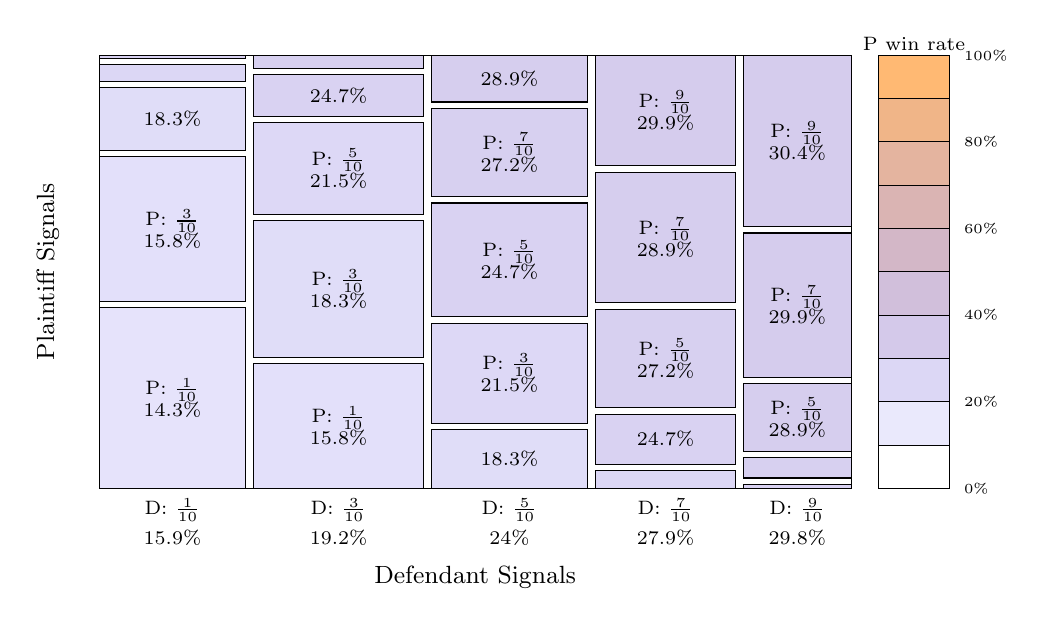
\begin{tikzpicture}
\newcommand{\DFractionOffset}{0.4}
\newcommand{\AxisLabelYAdjust}{-0.235}
\draw[draw=black] (0.6,2) rectangle (10.15,7.5);
\draw[fill=blue!86!orange!14!white!83!white, draw=black] (0.6,2) rectangle (2.4618,4.2924);
\draw (1.5309194840659774, 3.146194633205024) node[font=\scriptsize, text=black, align=center] {P: $\frac{1}{10}$\\ 14.3\%};
\draw[fill=blue!84!orange!16!white!83!white, draw=black] (0.6,4.3724) rectangle (2.4618,6.2099);
\draw (1.5309194840659774, 5.291142678996511) node[font=\scriptsize, text=black, align=center] {P: $\frac{3}{10}$\\ 15.8\%};
\draw[fill=blue!82!orange!18!white!82!white, draw=black] (0.6,6.2899) rectangle (2.4618,7.0878);
\draw (1.5309194840659774, 6.6888360761175925) node[font=\scriptsize, text=black, align=center] {18.3\%};
\draw[fill=blue!78!orange!22!white!81!white, draw=black] (0.6,7.1678) rectangle (2.4618,7.3817);
\draw[fill=blue!75!orange!25!white!80!white, draw=black] (0.6,7.4617) rectangle (2.4618,7.5);
\draw (1.5309194840659774, 1.6) node[anchor=north, font=\scriptsize, text=black] {15.9\%};
\draw (1.5309194840659774, {1.6 + \DFractionOffset}) node[anchor=north, font=\scriptsize, text=black] {D: $\frac{1}{10}$};
\draw[fill=blue!84!orange!16!white!83!white, draw=black] (2.5618,2) rectangle (4.7186,3.5862);
\draw (3.6402301083554898, 2.793112462563035) node[font=\scriptsize, text=black, align=center] {P: $\frac{1}{10}$\\ 15.8\%};
\draw[fill=blue!82!orange!18!white!82!white, draw=black] (2.5618,3.6662) rectangle (4.7186,5.398);
\draw (3.6402301083554898, 4.532103892841421) node[font=\scriptsize, text=black, align=center] {P: $\frac{3}{10}$\\ 18.3\%};
\draw[fill=blue!79!orange!21!white!81!white, draw=black] (2.5618,5.478) rectangle (4.7186,6.6479);
\draw (3.6402301083554898, 6.062955588639673) node[font=\scriptsize, text=black, align=center] {P: $\frac{5}{10}$\\ 21.5\%};
\draw[fill=blue!75!orange!25!white!80!white, draw=black] (2.5618,6.7279) rectangle (4.7186,7.2568);
\draw (3.6402301083554898, 6.992357986219307) node[font=\scriptsize, text=black, align=center] {24.7\%};
\draw[fill=blue!73!orange!27!white!79!white, draw=black] (2.5618,7.3368) rectangle (4.7186,7.5);
\draw (3.6402301083554898, 1.6) node[anchor=north, font=\scriptsize, text=black] {19.2\%};
\draw (3.6402301083554898, {1.6 + \DFractionOffset}) node[anchor=north, font=\scriptsize, text=black] {D: $\frac{3}{10}$};
\draw[fill=blue!82!orange!18!white!82!white, draw=black] (4.8186,2) rectangle (6.8038,2.7483);
\draw (5.811232644027941, 2.3741454171078646) node[font=\scriptsize, text=black, align=center] {18.3\%};
\draw[fill=blue!79!orange!21!white!81!white, draw=black] (4.8186,2.8283) rectangle (6.8038,4.0993);
\draw (5.811232644027941, 3.463815884733301) node[font=\scriptsize, text=black, align=center] {P: $\frac{3}{10}$\\ 21.5\%};
\draw[fill=blue!75!orange!25!white!80!white, draw=black] (4.8186,4.1793) rectangle (6.8038,5.6243);
\draw (5.811232644027941, 4.901821723594678) node[font=\scriptsize, text=black, align=center] {P: $\frac{5}{10}$\\ 24.7\%};
\draw[fill=blue!73!orange!27!white!79!white, draw=black] (4.8186,5.7043) rectangle (6.8038,6.8275);
\draw (5.811232644027941, 6.265903805209543) node[font=\scriptsize, text=black, align=center] {P: $\frac{7}{10}$\\ 27.2\%};
\draw[fill=blue!71!orange!29!white!78!white, draw=black] (4.8186,6.9075) rectangle (6.8038,7.5);
\draw (5.811232644027941, 7.203752549240302) node[font=\scriptsize, text=black, align=center] {28.9\%};
\draw (5.811232644027941, 1.6) node[anchor=north, font=\scriptsize, text=black] {24\%};
\draw (5.811232644027941, {1.6 + \DFractionOffset}) node[anchor=north, font=\scriptsize, text=black] {D: $\frac{5}{10}$};
\draw[fill=blue!78!orange!22!white!81!white, draw=black] (6.9038,2) rectangle (8.6849,2.2236);
\draw[fill=blue!75!orange!25!white!80!white, draw=black] (6.9038,2.3036) rectangle (8.6849,2.9441);
\draw (7.79439115866038, 2.623849485869879) node[font=\scriptsize, text=black, align=center] {24.7\%};
\draw[fill=blue!73!orange!27!white!79!white, draw=black] (6.9038,3.0241) rectangle (8.6849,4.276);
\draw (7.79439115866038, 3.6500211572461767) node[font=\scriptsize, text=black, align=center] {P: $\frac{5}{10}$\\ 27.2\%};
\draw[fill=blue!71!orange!29!white!78!white, draw=black] (6.9038,4.356) rectangle (8.6849,6.0165);
\draw (7.79439115866038, 5.186219956171058) node[font=\scriptsize, text=black, align=center] {P: $\frac{7}{10}$\\ 28.9\%};
\draw[fill=blue!70!orange!30!white!78!white, draw=black] (6.9038,6.0965) rectangle (8.6849,7.5);
\draw (7.79439115866038, 6.798226587872119) node[font=\scriptsize, text=black, align=center] {P: $\frac{9}{10}$\\ 29.9\%};
\draw (7.79439115866038, 1.6) node[anchor=north, font=\scriptsize, text=black] {27.9\%};
\draw (7.79439115866038, {1.6 + \DFractionOffset}) node[anchor=north, font=\scriptsize, text=black] {D: $\frac{7}{10}$};
\draw[fill=blue!75!orange!25!white!80!white, draw=black] (8.7849,2) rectangle (10.15,2.0522);
\draw[fill=blue!73!orange!27!white!79!white, draw=black] (8.7849,2.1322) rectangle (10.15,2.3901);
\draw[fill=blue!71!orange!29!white!78!white, draw=black] (8.7849,2.4701) rectangle (10.15,3.3318);
\draw (9.46746913892195, 2.900919670829747) node[font=\scriptsize, text=black, align=center] {P: $\frac{5}{10}$\\ 28.9\%};
\draw[fill=blue!70!orange!30!white!78!white, draw=black] (8.7849,3.4118) rectangle (10.15,5.2431);
\draw (9.46746913892195, 4.327409534358061) node[font=\scriptsize, text=black, align=center] {P: $\frac{7}{10}$\\ 29.9\%};
\draw[fill=blue!70!orange!30!white!78!white, draw=black] (8.7849,5.3231) rectangle (10.15,7.5);
\draw (9.46746913892195, 6.411531897151555) node[font=\scriptsize, text=black, align=center] {P: $\frac{9}{10}$\\ 30.4\%};
\draw (9.46746913892195, 1.6) node[anchor=north, font=\scriptsize, text=black] {29.8\%};
\draw (9.46746913892195, {1.6 + \DFractionOffset}) node[anchor=north, font=\scriptsize, text=black] {D: $\frac{9}{10}$};
\node[font=\small, text=black] at (5.375, {1.1 + \AxisLabelYAdjust}) {Defendant Signals};
\node[font=\small, text=black, rotate=90] at (-0.050000000000000044, 4.75) {Plaintiff Signals};
\draw[draw=black] (10.5,2) rectangle (11.4,7.5);
\draw (10.95, 7.65) node[font=\scriptsize, text=black] {P win rate};
\draw[fill=blue!100!orange!0!white!88!white, draw=black] (10.5,2) rectangle (11.4,2.55);
\draw[fill=blue!89!orange!11!white!84!white, draw=black] (10.5,2.55) rectangle (11.4,3.1);
\draw[fill=blue!78!orange!22!white!81!white, draw=black] (10.5,3.1) rectangle (11.4,3.65);
\draw[fill=blue!67!orange!33!white!77!white, draw=black] (10.5,3.65) rectangle (11.4,4.2);
\draw[fill=blue!56!orange!44!white!73!white, draw=black] (10.5,4.2) rectangle (11.4,4.75);
\draw[fill=blue!44!orange!56!white!70!white, draw=black] (10.5,4.75) rectangle (11.4,5.3);
\draw[fill=blue!33!orange!67!white!66!white, draw=black] (10.5,5.3) rectangle (11.4,5.85);
\draw[fill=blue!22!orange!78!white!62!white, draw=black] (10.5,5.85) rectangle (11.4,6.4);
\draw[fill=blue!11!orange!89!white!59!white, draw=black] (10.5,6.4) rectangle (11.4,6.95);
\draw[fill=blue!0!orange!100!white!55!white, draw=black] (10.5,6.95) rectangle (11.4,7.5);
\draw (11.46, 2) node[anchor=west, font=\tiny, text=black] {0\%};
\draw (11.46, 3.1) node[anchor=west, font=\tiny, text=black] {20\%};
\draw (11.46, 4.2) node[anchor=west, font=\tiny, text=black] {40\%};
\draw (11.46, 5.3) node[anchor=west, font=\tiny, text=black] {60\%};
\draw (11.46, 6.4) node[anchor=west, font=\tiny, text=black] {80\%};
\draw (11.46, 7.5) node[anchor=west, font=\tiny, text=black] {100\%};


\end{tikzpicture}
\end{document}